\externaldocument{../appendix/chapter_app}
\externaldocument{../4/chapter_algorithm}
\startchapter{Evaluation}
\label{chapter:Exp}
This evaluation aimed to experimentally evaluate the model for communication analysis and the identification algorithms. The evaluation only focus on evaluating the correctness and efficiency of the model and algorithm. User case study is not included in this thesis and can be the future work. The feature prototype implementation is not evaluated and can be part of the user case study. In this section, I describe the design of the evaluation.  Then the results of the experiment evaluation are provided and concluded.

\subsection{Experiment Evaluation Design}
Two experiments are conducted for this evaluation.  All the programs in these two experiments were written in C++ and the source code can be found in Section\ref{expcode}. Our search partner DRDC provided the captured traces, the used .dll files and  the source code of the programs for the experiments.

In the first experiment, two programs communicated with each other through a synchronous Named pipe channel. One of the programs acted as the Named pipe server while the other as the client. Figure\ref{exp1} is the sequence diagram of the interaction between the server and client. Traces were captured while these two program were running and interacting. The two captured traces are analysis as dual\_trace exp1 in this experiment. 

\begin{figure}[H]
\centerline{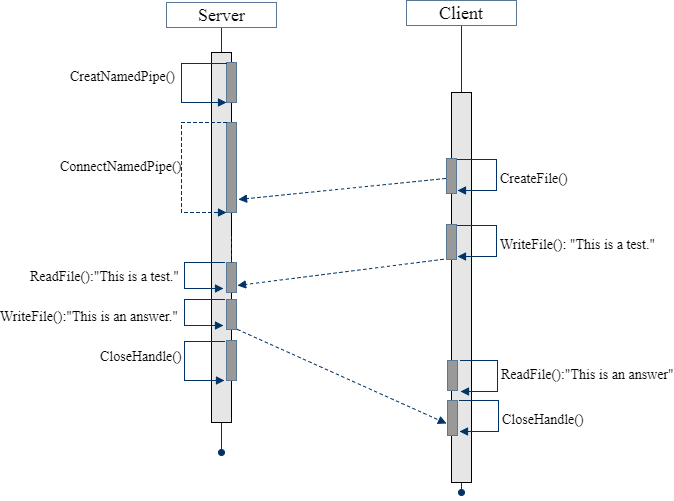
\includegraphics[scale=0.7]{Figures/exp1}}
 \caption{Sequence Diagram of Experiment 1}
\label{exp1}
\end{figure}

In the second experiment, one program was running as the Named pipe server, while two other programs as the Named pipe clients connected to this server. Those two clients (client 1 and client 2) use the identical program but run in sequence. Figure\ref{exp2} is the sequence diagram of  the interaction among the server and clients. Three traces were captured at the time when these three programs were running and interacting. These three traces generated two dua\_traces, exp2.1 and exp2.2, exp2.1 consist of traces of server and client 1 and exp2.2 consist of traces of server and client 2. Both dual\_traces were being analysed in this experiment.

\begin{figure}[H]
\centerline{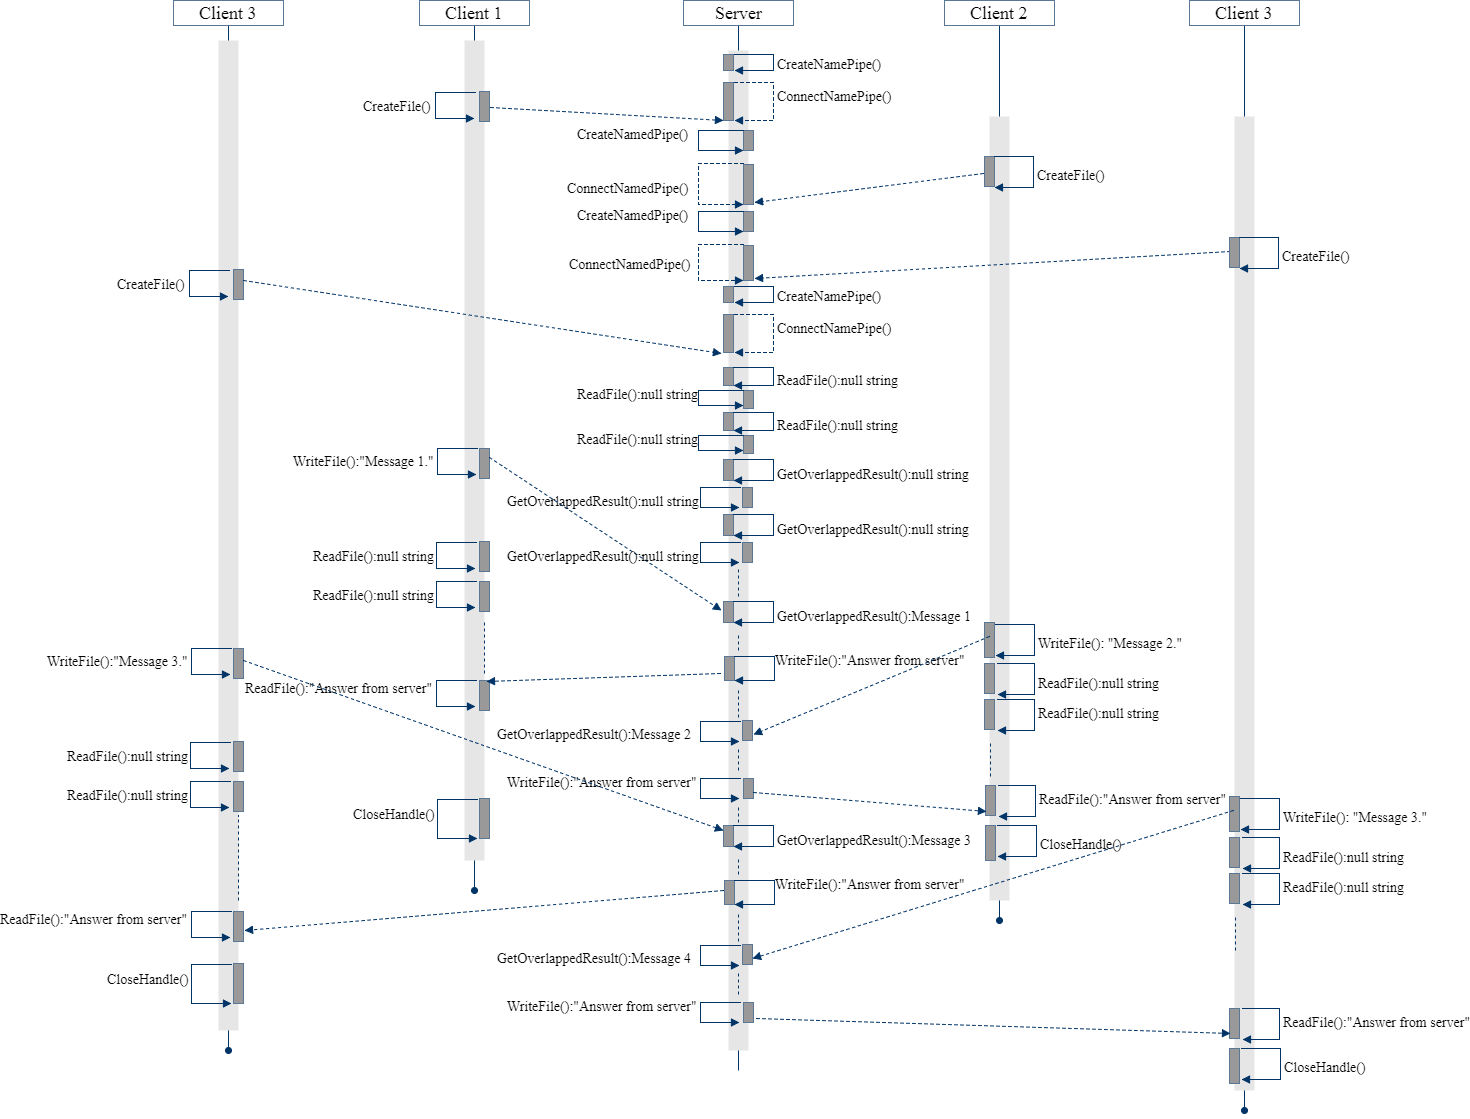
\includegraphics[scale=0.6]{Figures/exp2}}
 \caption{Sequence Diagram of Experiment 2}
\label{exp2}
\end{figure}

I used the implemented feature on Atlantis to conduct the dual\_traces analysis for the experiments. ``Communication identification" was conducted for all dual\_traces. The result of these two experiments is discussed in next section. 

\subsection{Result and Conclusion}
The identification result and the processing time of the identifications of each experiment are listed in Table\ref{expresult}. All communications in the dual\_traces are being successfully identified. However, dual to the channel id and transmitted data of the communication between server and client 1 was identical to those of the communication  between server and client 2. There is one false negative error in exp2.1 and one in exp2.2 which is align to the explanation in Section\ref{streammatch}. The dual\_traces being analysed is relatively small, so that the processing times of the identification are acceptable. Fortunately, according to the time complexity of the main algorithm of the identification which is O(N+M), the processing time will only grow linearly corresponding to the size of the dual\_trace.

    \begin{table}[H]
        \centering
        \caption{Communication Identification Experiment Result}
        \label{expresult}
        \begin{threeparttable}
        \begin{tabular}{|c|c|c|c|c|}
            \hline
            \textbf{Dual\_trace}&\textbf{Actual}\tnote{1}& \textbf{Success}\tnote{2}& \textbf{Error}\tnote{3} & \textbf{Processing Time(s)} \\
             \hline
             \textbf{exp1} &1&1&0&0.0\\
            \hline
             \textbf{exp2.1}&1&1&1&    0.0\\
            \hline
             \textbf{exp2.2}&1&1&1&0.0\\
            \hline
        \end{tabular}
        \begin{tablenotes}
            \item[1] Actual communication number in this dual\_trace
            \item[2] Success identified communication number of this dual\_trace
            \item[2] Error identified communication number of this dual\_trace, including false negative and false positive errors
        \end{tablenotes}
        \end{threeparttable}
    \end{table}




